\chapter{Laporan Database}
\section{Create Aplication dan From A File Data Min 50 Record}
\par
\begin{enumerate}
    \item Pertama kunjungi Aplikasi APEX \textit{https://apex.oracle.com/} 
    \item Kemudian Masuk pada APEX nya dengan Melakukan \textit{SIGN IN} jika tidak memiliki akun maka lakukan \textit{SIGN UP}.
    \item Lalu jika sudah masuk Aplikasi APEX nya maka akan muncul seperti gambar dibawah.
    \begin{figure}[!htbp]
\centering
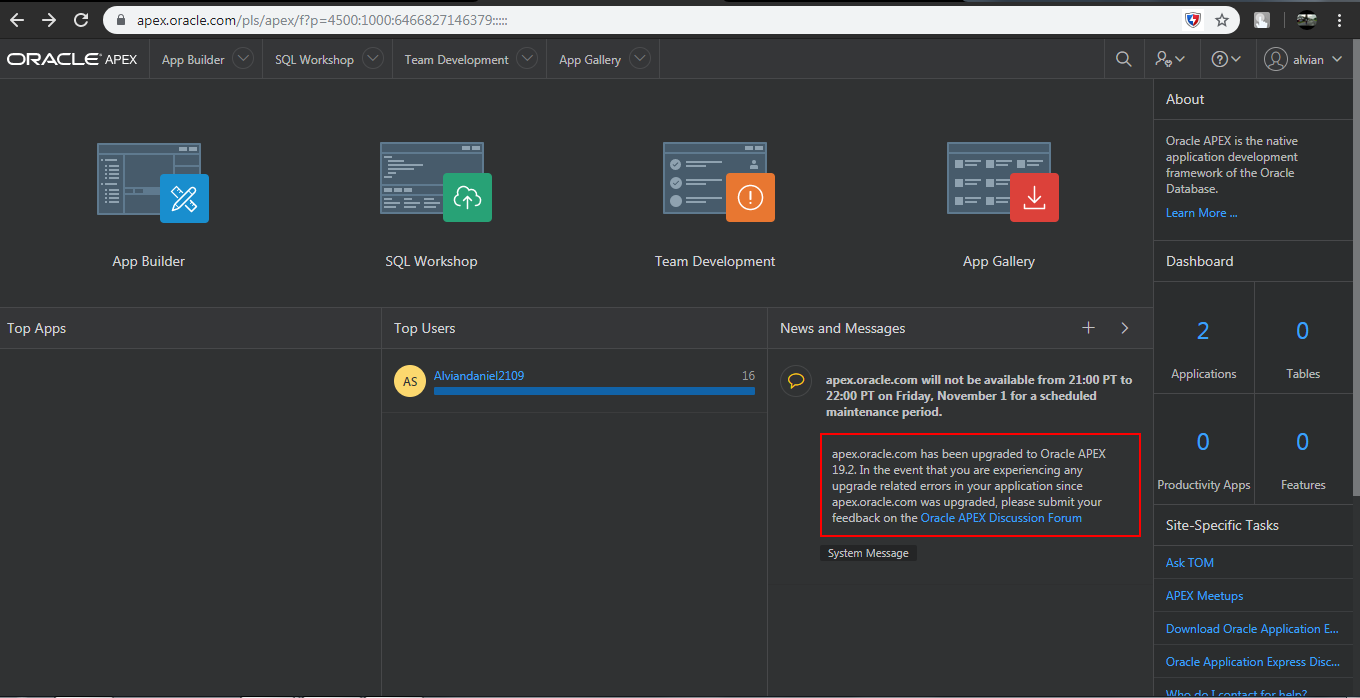
\includegraphics[width=10cm,height=9cm]{figures/A.PNG}
\caption{Menu Awal}
\label{penanda}
\end{figure}
    \item Kemudian Masuk Ke \textit{APP BUILDER}.
\begin{figure}[!htbp]
\centering
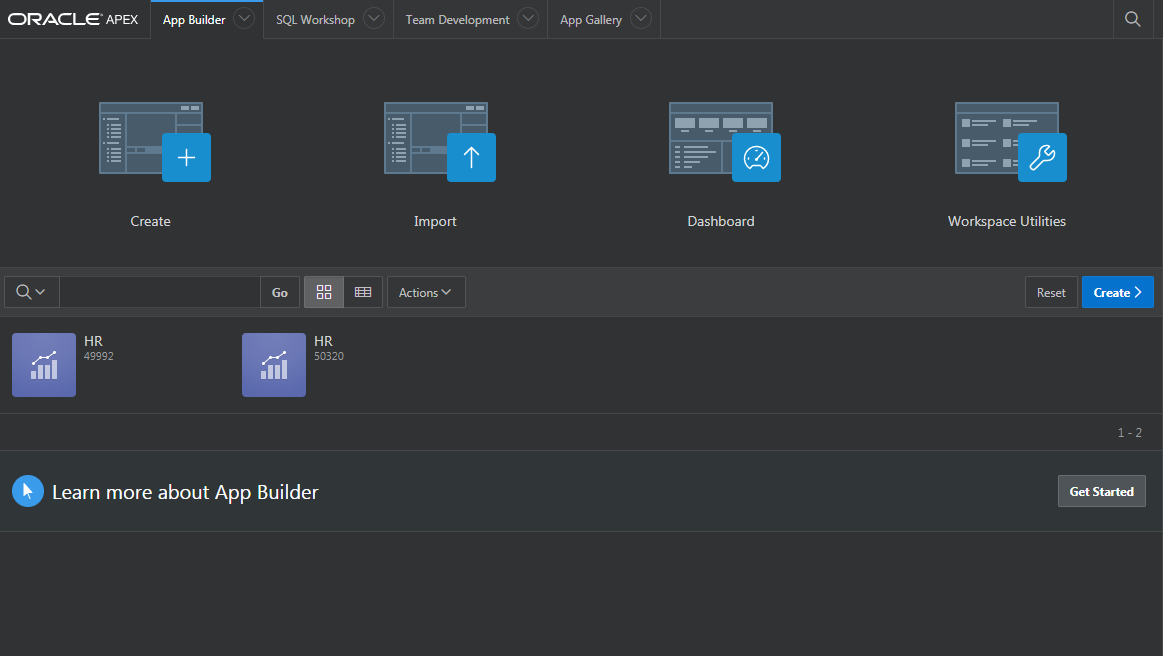
\includegraphics[width=11cm,height=9cm]{figures/B.PNG}
\caption{Menu APP BUILDER}
\label{penanda}
\end{figure}
    \item Masuk ke Halaman \textbf{Create}
\begin{figure}[!htbp]
\centering
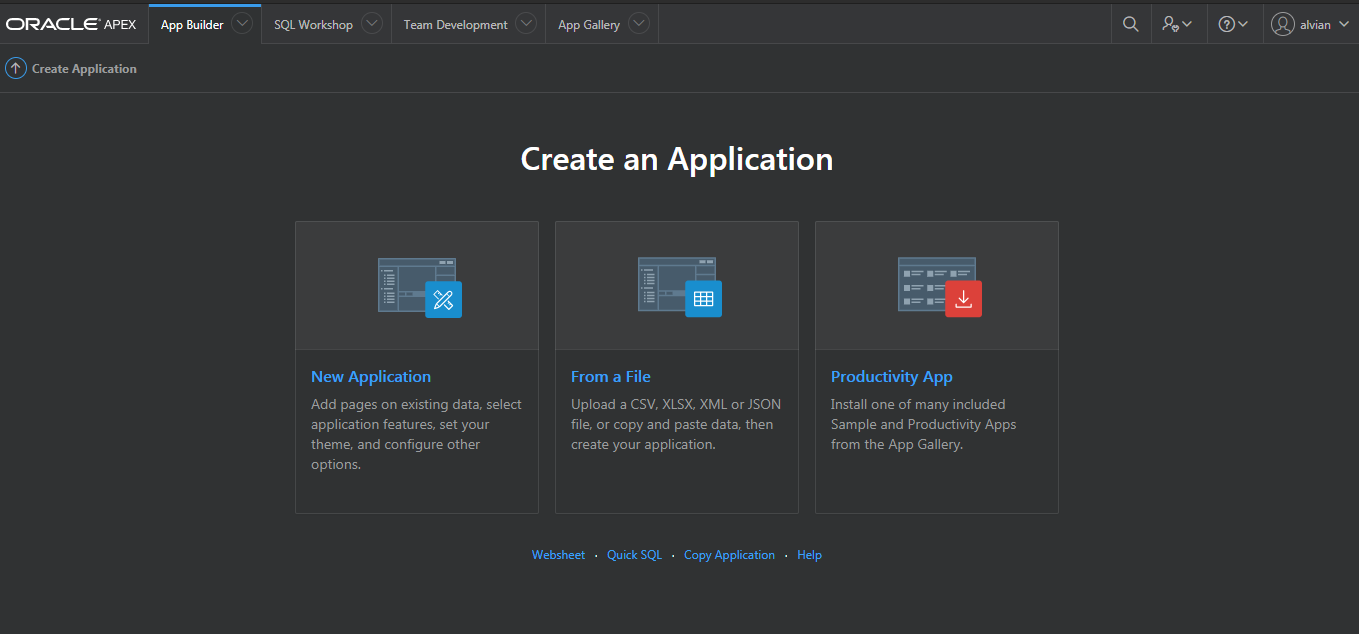
\includegraphics[width=11cm,height=9cm]{figures/C.PNG}
\caption{Menu Create}
\label{penanda}
\end{figure}
    \item Jika sudah maka Klik \textit{From a file}
\begin{figure}[!htbp]
\centering
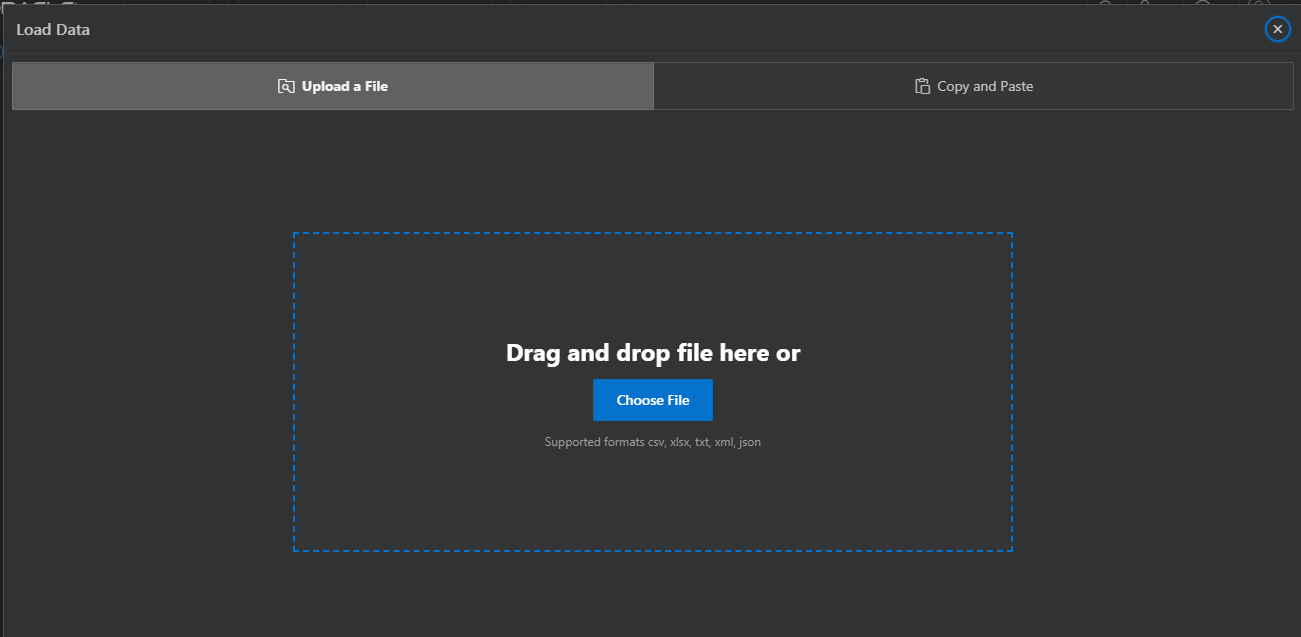
\includegraphics[width=10cm,height=8cm]{figures/D.PNG}
\caption{From a file}
\label{penanda}
\end{figure}
\item Kemudian Masukkan data anda, disini saya memasukkan data yang lebih dari 50 record yaitu data \textit{Data Mahasiswa D4 TI Politeknik Pos Indonesia} 
\item Akan muncul gambar seperti dibawah ini.
\begin{figure}[!htbp]
\centering
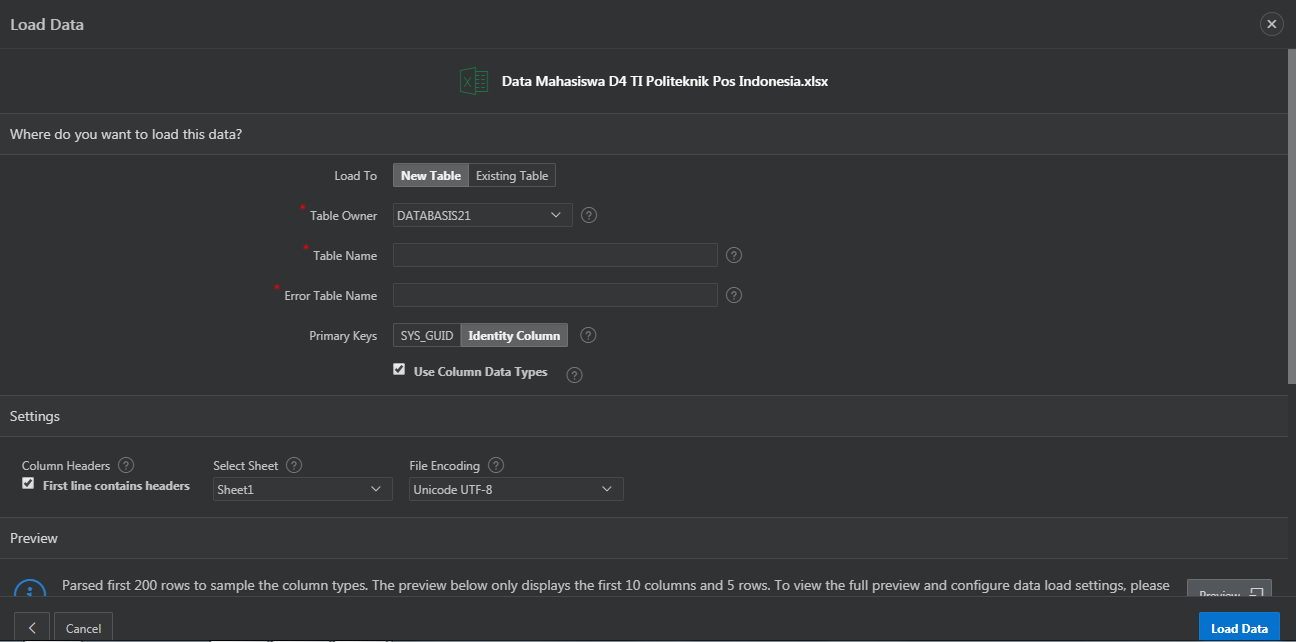
\includegraphics[width=10cm,height=8cm]{figures/E.PNG}
\caption{Upload File}
\label{penanda}
\end{figure}
\item Lalu Masukkan \textbf{Nama Table,} jika Sudah tekan Configure pada bagian bawah Name table, Kemudian Save Change.
\begin{figure}[!htbp]
\centering
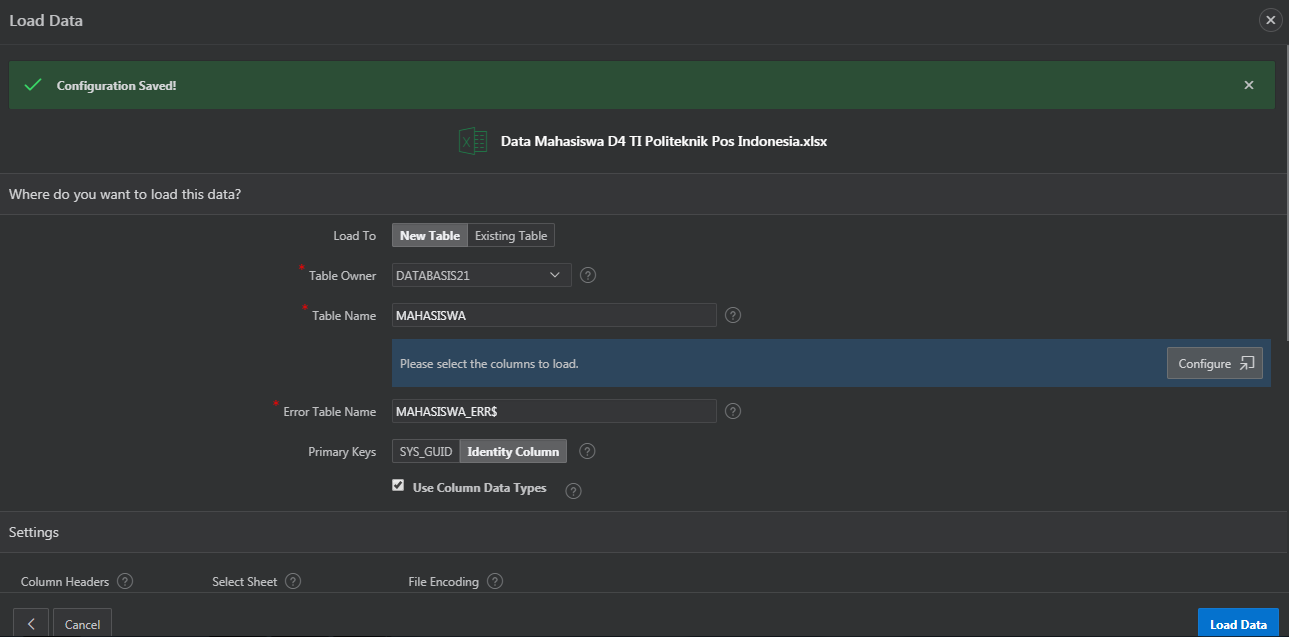
\includegraphics[width=10cm,height=8cm]{figures/F.PNG}
\caption{Save Changes}
\label{penanda}
\end{figure}
\item Tekan Load Data.
\begin{figure}[!htbp]
\centering
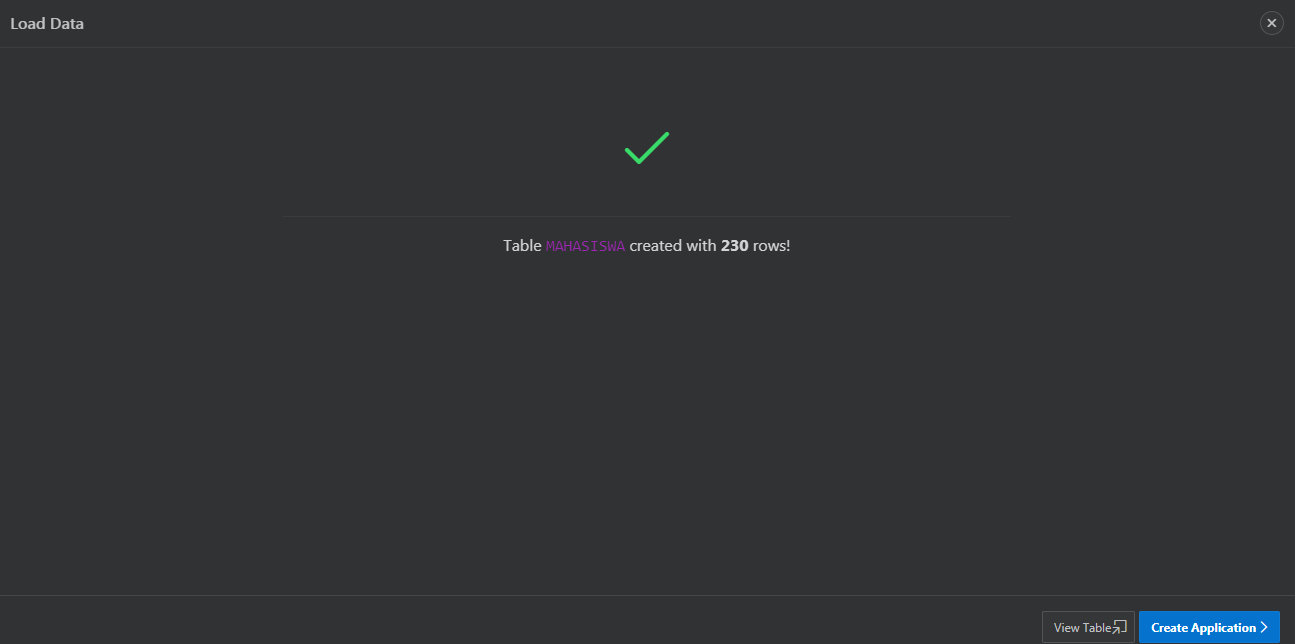
\includegraphics[width=10cm,height=8cm]{figures/G.PNG}
\caption{load Data}
\label{penanda}
\end{figure}
\item nah disini, ada 230 rows yang artinya ada 230 record data masuk pada data tersebut.
\item Kemudian Klik \textit{Create Application.}
\begin{figure}[!htbp]
\centering
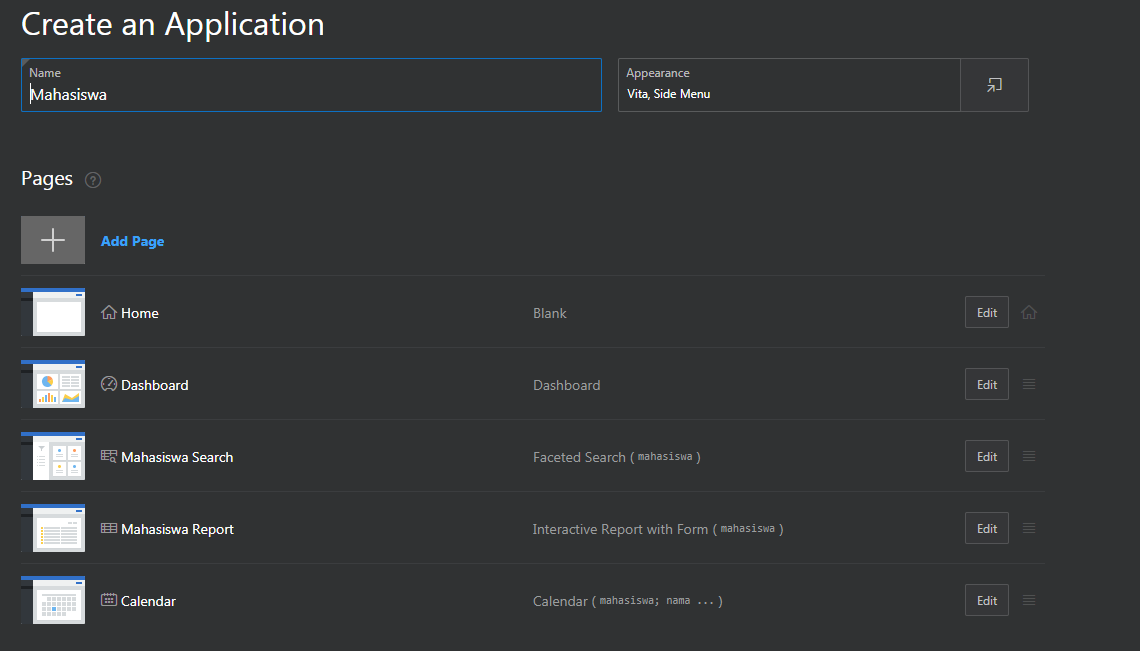
\includegraphics[width=10cm,height=8cm]{figures/H.PNG}
\caption{Create Application}
\label{penanda}
\end{figure}
\item Jika sudah maka klik \textit{Create Application}
\item Loading.
\begin{figure}[!htbp]
\centering
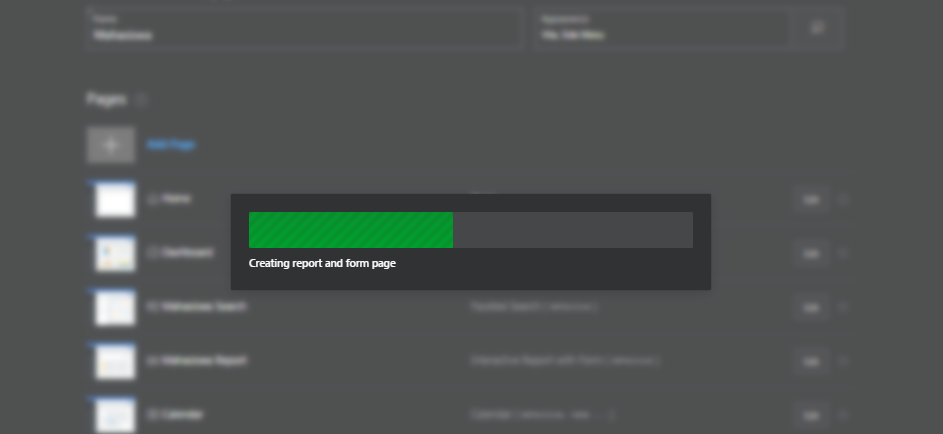
\includegraphics[width=10cm,height=9cm]{figures/I.PNG}
\caption{Loading}
\label{penanda}
\end{figure}
\item Klik Run Application.
\begin{figure}[!htbp]
\centering
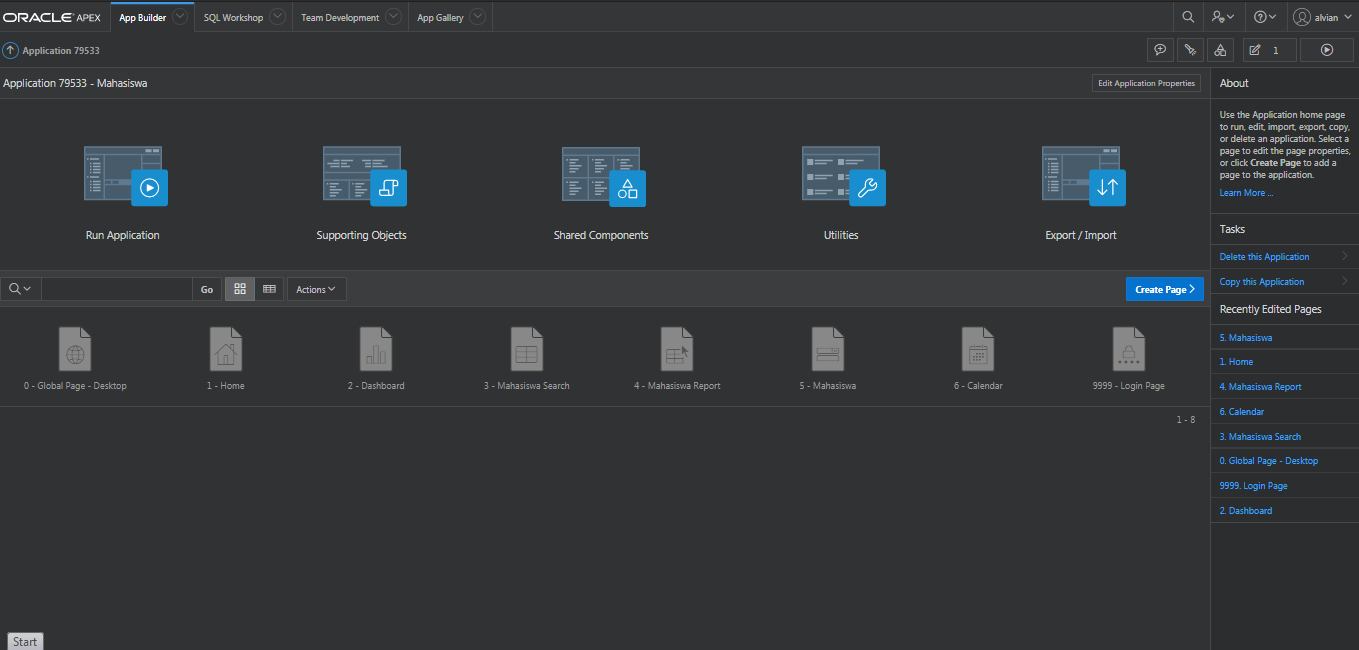
\includegraphics[width=10cm,height=8cm]{figures/J.PNG}
\caption{Run Application}
\label{penanda}
\end{figure}
\item Kemudian Lakukan Login pada Halaman utama, \textit{masukkan username dan password APEX} anda.
\begin{figure}[!htbp]
\centering
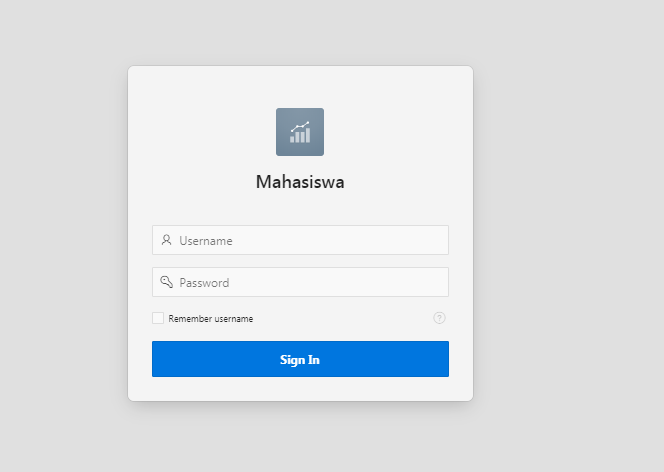
\includegraphics[width=10cm,height=8cm]{figures/K.PNG}
\caption{Login}
\label{penanda}
\end{figure}
\item Setelah melakukan Login Maka akan masuk pada halaman utama Aplikasi anda seperti dibawah ini.
\begin{figure}[!htbp]
\centering
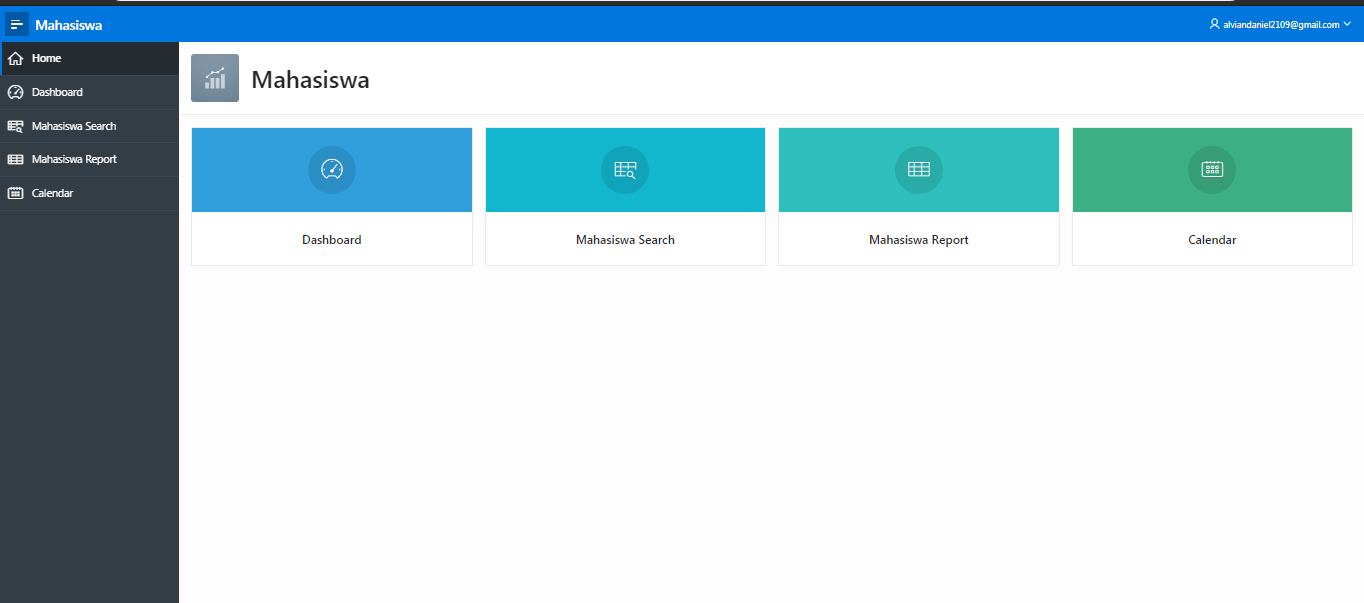
\includegraphics[width=10cm,height=8cm]{figures/L.PNG}
\caption{Halaman Utama}
\label{penanda}
\end{figure}
\item Kemudian Anda dapat melihat Record data anda tadi dalam Report.
\begin{figure}[!htbp]
\centering
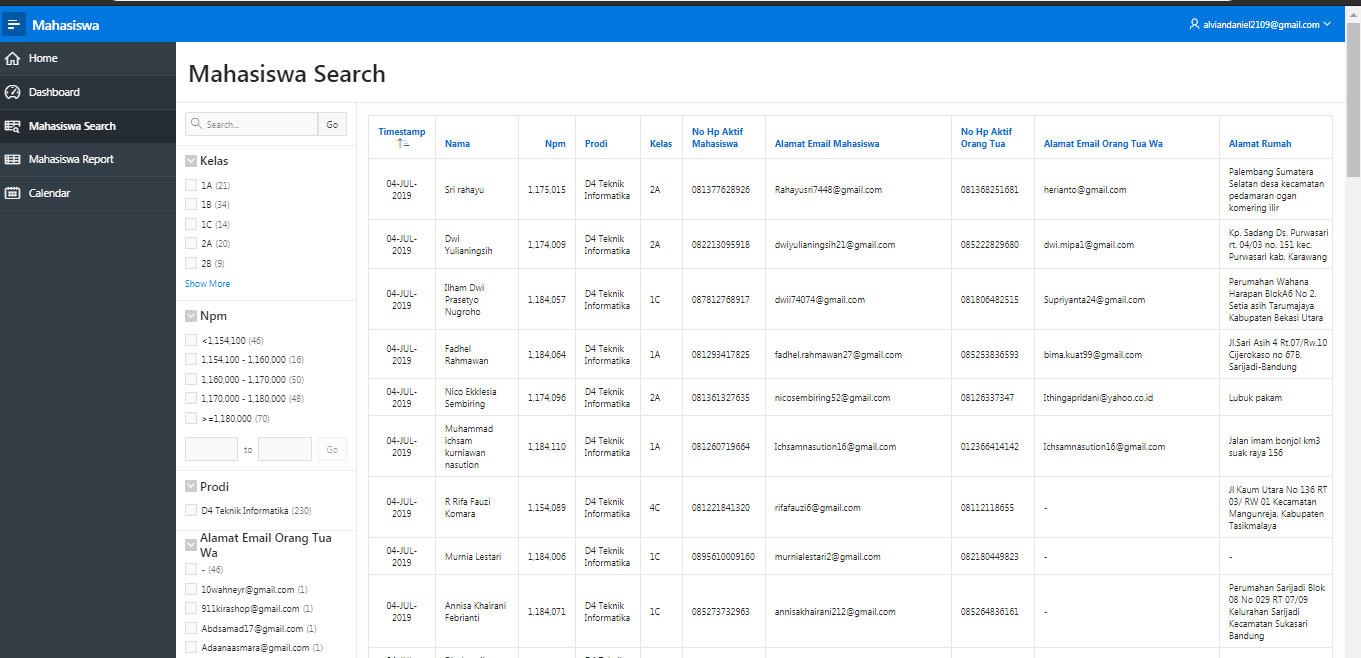
\includegraphics[width=10cm,height=8cm]{figures/M.PNG}
\caption{Report}
\label{penanda}
\end{figure}
\item dan anda telah berhasil melakukan Create dan From a file pada APEX
\end{enumerate}
